% !TeX root = ../main.tex
% Add the above to each chapter to make compiling the PDF easier in some editors.

\chapter{Introduction}\label{chapter:introduction}

\section{Background}
Internet of Things (IoT) has become an emerging technology with the power of low priced computational units and the cloud technology. There are thousands of different examples in the real world which targets both the end-users and the industry. 

The problem with the current state of art is requirement of tremendous time investment by the developers. The developers need to spend this time to develop both embedded software and web services to serve their goal. The most of this can be spent on already implemented functionalities in different projects with slight differences.

In IoT practical course offered during winter semester 2017/18 in Technical University of Munich, a generic and practical platform for single board computers is built. The idea of building a generic and practical platform to be used in the scope of IoT to prototype and develop can also be realized for the web services. Moreover, the open source development of the hardware platform can be sustained and expanded to have full support and integration with this web services platform. By using two platforms in parallel, prototyping the projects in the scope of IoT will require much less time for the developer.

In most cases, the applications have similar capability needs in their required web-services with some little customization. The most basic capabilities, which any web services should have, can be listed as;
\begin{itemize}
  \item Receiving data,
  \item Serving data,
  \item Applying rules on gathered data when an event occurs,
  \item User authentication and authorization,
  \item Data isolation.
\end{itemize}
 Furthermore, they may need to support multiple protocols at the same time for accessing and modifying the same data since these web services should be accessible by different platforms. Although multiple protocols are used at the same time, the choice of protocols is always similar. 

 Message Queue Telemetry Transport (MQTT), Constrained Application Protocol (CoAP) and Hypertext Transfer Protocol (HTTP) in Representational State Transfer (REST) architectural style are the most used protocols in the area of IoT \cite{8246418,8070130}. Machine to machine (M2M) communications between wireless sensor network nodes and web application server are done through CoAP since they are resource-constrained devices regarding the power source, the memory, and the network availability. Also, CoAP is designed to be used in these kinds of constrained networks. If a node needs to send a message to multiple different nodes at the same time, MQTT is preferred since it is a lightweight publish-subscribe based messaging protocol and supports one-to-many communication \cite{mqtt}. Devices such as smartphones and personal computers which are not in a constrained network use HTTP in a RESTful way to monitor the gathered data, to start events or both.

 The common trait of all these protocols is to be highly generic to support any needs of the developer on their communication through the internet. On the other hand, the required functionalities of web services that are used in the area of IoT diverge from each other with only a little difference. Interoperability of sensors, actuators, machine to machine (M2M) communication and context-aware services is the primary concern of IoT \cite{6651222}. 

To point out the challanges in the current state of art within an example, a corporate comany which delivers IoT solutions for the factory automation systems can be taken into account. This corporate company customizes their own system to match with the needs of their customers. In scope of of the web services, this customization may be addition of a new protocol, support of different type of devices, implementation of brand-new feautre or integration of features that are already implmented in the past for another customer.

All of these customization may lead challanges which wil end up with hiring new developers or losing the potential customers. A Platform as a Service (PaaS) can be defined to develop and to maintain custom web services in IoT domain by using predefined and parameterized building blocks to give developers a fast and practical environment to ease and erase these challanges.

\section{Proposed Solution}

This master thesis aims to build a platform for the developers in the area of IoT to build their web services within a generic and practical development environment. An abstraction of all functionalities of the web services that are needed for any IoT project would help to achieve this generic platform. On the other hand, the genericity would be a challenge to accomplish the practicality goal. So to maintain practicality, the resulting platform shall be definite and comprehensive enough to support any IoT project and the web services used in other areas shall not be a concern. 

While designing web services that will be used in these scenarios as well as others, some design concerns must be taken into account by the developers. The techniques and architecture to enable communication between all necessary nodes, the format for the data that will be stored, how and when data will be served can be considered as the main design concerns \cite{6651222}. After the design phase of the system has been finished, the design shall be easily implemented to make the web services up and to run them. 
There exist different options with different practicality levels to implement the designed web services in the platform. 

The resulting platform will provide solutions in different degrees for the practicality challanges and problems in IoT domain. These challanges and problems can be listed as following;

\begin{enumerate}
	\item The need of the time investment
	\item The reimplementation of already implemented functionality
	\item The deployment of the system
	\item The maintanance of the system
	\item Requirement of the technical background
	\item Different technologies to define same functionalities
\end{enumerate}


The platform shall render a practical and easy to learn web user interface (UI) for the hobby users with a less technical background as in the first scenario. The data, the users, the rules and the web services, which are owned by the platform user, will be easily accessible and mutable by the platform user in the UI. The platform users will quickly adapt even if they have little technical background since the system provides building blocks to connect with each other by using the most common user experience (UX) elements such as drag-drop objects, wires, and forms. The power users such as in the second and third scenario are provided with application program interface (API) to use any functionality of the platform through HTTP requests and Internet of Things Easy Query Language (IoTeQL) to manipulate their data and rules as well as the UI for their basic operations on their system. With the help of API and IoTeQL, existing systems such as the third scenario can be transferred to the platform quickly with the help of a script. Moreover, the scenarios similar to the third scenario, which need to provide multiple services with a little customization, can be done quickly by using reusable components that will be described later in this section.

The platform shall store the data of the web applications of the platform users in an easily accessible, organizable and modifiable way without loss of genericity. M. G. Kibria et al. proposed that a semantic ontology which declares every device as objects on the gateways can be used for the energy efficiency \cite{7993747}. N. Lee and H. Lee also suggested an IoT service architecture that provides services with an object gateway \cite{6884496}. Although the device objectification on ontologies is a reliable method to store the data of the real world devices in IoT services; the management of read-write access to the objects, the evaluation of the gathered data and the methods for the service of these data are the topics that need to be covered to build a generic and practical platform that serves any needs of IoT.

To build business logic and define evaluation methods on the ontologies; the rules, which are in if-then form decision-making tools, must be introduced in the platform. The rules function like a chain of blocks, where each does a small fraction of the functionality while interpreting the logic.  There are different types of blocks that each has a different function in the rule handling. The limited toolbox of generic rule blocks also preserves the practicality for the users since they do not need to master a vast pool of different block types.

The users defined for any web services should be reusable among the other web services. Therefore, the newly founded business similar to the second scenario will be able to serve new services to their existing users effortlessly. Additionally, the user pools of the web services should be separated from the ontologies. Therefore, an ontology of a web service can be cloned to be used in a different web service efficiently without any user that the previous web service uses. Hence, the company in the third scenario can provide their services to its new customers by separating previous customers with little or no work.

Furthermore, the user pools can have different user confirmation level. These confirmation levels define when the web services user needs to confirm whether they agree on the usage of their data in the web services, who can access the objects that are owned by a web service user and how to use the user information. The user confirmation levels achieve the ease of handling of user data needed for the platform users who are building web services in different countries that have different user data protection regulations.

The platform shall provide support for the development using the most popular web services protocols in IoT such as REST, CoAP and MQTT. On the other hand, it shall have the abstraction to support any future protocols that will solve problems in the IoT area. By virtue of the separation of the ontologies, the user pools, and the web services protocols; the platform user can switch between or easily unite multiple protocols, even they are newly introduced.

To achieve this PaaS that enables a fast, practical, accessible and generic environment that can support any IoT developer, different subsystems that handle different objectives in the system must be defined. By having different subsystems,  isolation of information and a system that scales only its required subsystems can be succeeded. On the other hand, the challenge of interoperability between these subsystem occurs. In figure \ref{fig:architecture}, the architectural design of the system is shown.
\clearpage
\begin{figure}[h]
  \centering
  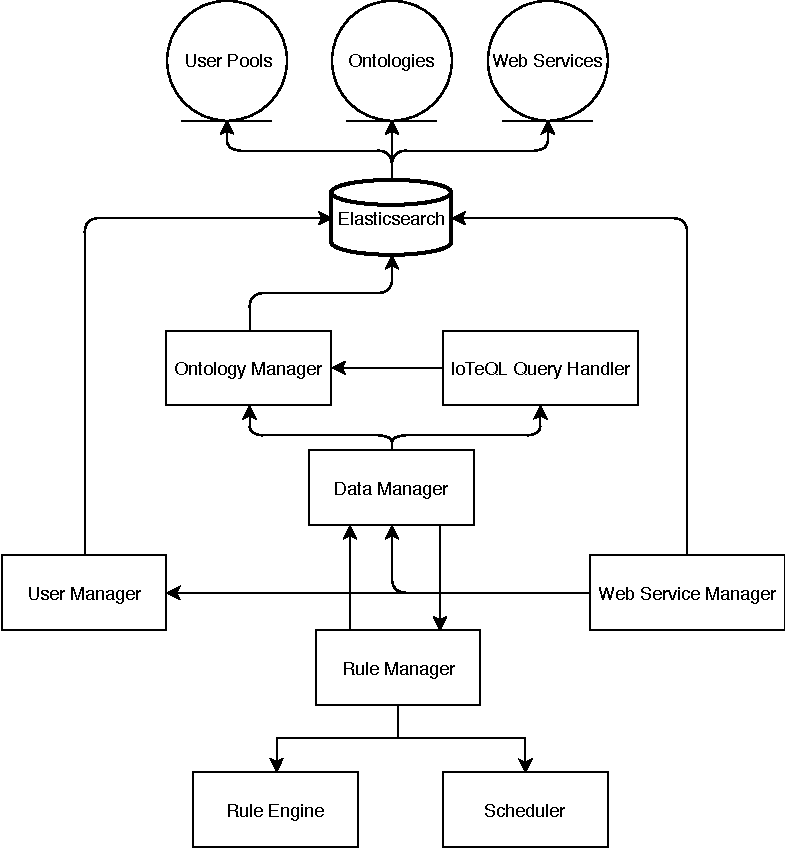
\includegraphics[width=0.7\textwidth,height=\textheight,keepaspectratio]{figures/high_level_architectural_diagram.pdf}
  \caption[Platform Architecture]{The high level architectural diagram of the platform}\label{fig:architecture}
\end{figure}

Each of the subsystems; the user manager, the data manager, the rule manager and the web services manager are dockerized and hosted in different computing units in the cloud infrastructure. Since they are isolated and loosely coupled with each other, they can autoscale individually behind a load balancer and expansion of the computational unit where it is needed can be achieved. Consequently, only the data manager will horizontally scale when the number of queries is increased, or only the rule manager will scale horizontally when the massive amount of scheduled rules is needed to be handled at the same time. A platform user can access all of the subsystems by their APIs, and the connector components of them act like adapter to interact with each other. Therefore, any change in any subsystem will not lead change in overall architecture. How to handle the interoperability challenges will be covered in the following chapters in details.


%\subsection{Data Manager}

%All the data that is defined by the platform user and the web service users is handled by the data manager and its components. Data manager uses Elasticsearch to store this data since its scalability, speed, resiliency, flexibility, powerful support to time-series and unstructured data and queries \cite{elastic, elastic_time}.

%Any data that will be used by the web services that are defined by the platform user are stored as ontologies in the platform. These ontologies store different types of components as follows:

%\begin{itemize}
%  \item Types
%  \item Figures
%  \item Objects
%  \item Groups
%  \item Rules
%\end{itemize}

%The data model of an ontology is defined by types and figures and the actual data is defined by objects and groups. Each type has a name and abstract meta-data about data fields such as requirement, name, and type which will be used while defining objects. A type can be inherited by another type, figure or can be used to define objects. The figures are just like types, but, with predefined data fields. The objects that are defined by using a figure cannot alter these predefined data fields other than the value given in the figures. Each figure cannot be inherited by a type and must inherit from a type. Each object is defined by using a type or a figure, represents the virtual state of a real-world object and can have concrete data, data series or rules that are defined in type or figure which the object inherits and return on-time calculated value in its fields. To state a property of an object, data fields can be used. On the other hand, data series are preferred to store a collection of the same type of data of the same object such as timestamped data of hourly energy consumption of a device. The groups are used to cluster objects and apply rules on objects as a cluster. The rules are chains of function blocks to apply on objects or groups when an event occurs. They are stored in ontologies with other components by the data manager. However, processing and handling of them are done by the rule manager. In the subsection \ref{ss:rule_manager}, the detailed information about rule structure will be given.

%Any ontology owned by a platform user can be shared with other platform users to work collaboratively. Nevertheless, the platform users that have no access to an ontology are not allowed to view or modify the ontology. As a result, the protection of business logic and private data will be preserved. The isolation of the ontologies is also handled by the data manager. 

%The created ontologies can only be organized and extended by a platform user. Any rules or object in an ontology will not function until the ontology is matched with a web service using the web service manager. Thus, an ontology that is not matched with any web service is considered offline and act like static data in the platform.

%To enable reusability of an ontology, they can be edited, cloned or taken offline. Moreover, they can be matched with multiple web services and any changes made using a web service will be available on other matched web services. Therefore, the data will be available in the platform user-defined system from any kind of network.

%The whole ontology can be defined in the practical and easy-to-learn user interface (UI) of the web application. However, the power users who want to transfer existing data models as ontologies to the platform with help of a script, to modify the ontology components that cannot be modified by the rules such as creating or removing rules with their own system or need to create a similar ontology with the small but core changes which would lead the loss of data when is done in UI can use Internet of Things Easy Query Language (IoTeQL) that is designed for querying the ontology model and enables all functionality of the ontology model for the needs of the user in a practical way. All queries on the ontologies are evaluated by the query engine component of the data manager. The detailed information and syntax of IoTeQL can be found in upcoming chapters. %TODO Chapter 


%\subsection{Rule Manager}
%\label{ss:rule_manager}

%To build business logic on the ontologies; the rules, which are if-then form decision-making tools, must be defined in the platform. The rules function like a chain of blocks, which each does a small fraction of the functionality while interpreting the logic. These blocks send and receive objects in JavaScript Object Notation (JSON) format between each other using their input and output ports. There are different types of blocks that each has a different function in the rule handling. In the following part, the blocks and their respective descriptions can be found.

%\begin{description}
%  \item [Nodes] are used to retrieve data from other components of the ontology. They can represent a type, a figure, an object or values in the data fields of the object. They are also directly accessible by the endpoints of a web service.
%  \item [Queries] are used to create a new object or to modify the existing ones. They can match with the objects as a whole or as part of them and outputs state of the whole object. 
%  \item [Sinks] are used to connect the rules to the web services. They are the exit points for the data to be sent through the web services.
%  \item [Sources] are also used to connect the rules to the web services. They are the entry points for the data received from the web services.
%  \item [Events] are used to run the rules when a condition satisfied. This condition can be satisfied by the time or other rule blocks. If the condition is time-based, they can run their respective rules with predefined value output at the scheduled times. If it is expected to be triggered by other function blocks, they must have a condition to apply on input and outputs input to its target when the condition is satisfied.
%  \item [Mappers] have a lambda function to apply every single element of the input and output elements which the function returns.
%  \item [Reducers] have a lambda function which does rolling computation to apply to sequential pairs of data series.
%  \item [Filters] have a lambda function which returns a boolean type value. They apply the lambda function to elements in the input and output elements which the function returns true.
%  \item [Zippers] are used to merge more than one inputs into a single output.
%  \item [Branchs] have more than one output ports and each output port have their respective condition. They forward their input to the output port or ports that conditions are satisfied.
%  \item [Functions] are used to do a customized modification on the input in a sequential programming way and output result when the capabilities of other blocks are not enough.
%\end{description}

% A web service triggers respective source in a rule on each request and returns the value received from sinks if it has one. The only way to run a rule is triggering its starting sink or event. Every rule block can have only one output port and can have more than one input ports except sinks and sources and are reusable with their target blocks by referencing them while creating a rule. With the power of reusable blocks, the platform user will not need to implement the rule parts that are already implemented in other rules.

%\subsection{User Manager}

%The web services that are defined by the platform user may have public or private endpoints. To be able to reach the private endpoints, the web service user must have correct access rights. The user pools can be defined by the platform user to manage access rights to private endpoints of the web services. The authorization rights, the user groups with assigned authorization rights and users which belong to one or more user groups and have personal information must be defined in a user pool. 

%The reason to keep the web services and the user pools separate is to escalate the reusability of the same user pool. The platform user may want to introduce new web services to his/her own system. In such a case, it would be undesirable for the web service users to create new accounts to use a new web service. Therefore, using the same user pool in both web services would be ideal. 

%The new user pools can be created and managed through the web application. The endpoints of the REST API of the user pool are also provided to the platform user. With help of these endpoints, they can integrate user creation and modification functions for their users in different user groups into their own system. 

%The user pools can also have different user confirmation level. These confirmation levels define when the web services user needs to confirm whether they agree on the usage of their data in the web services. The objects, that are owned by a web service user, cannot be accessed with the web services unless the permission is given. One time confirmation to use the user information in any web services which are created by the same platform user or the confirmation requirement before the start of using of any individual web services can be set by the platform user for each user pool. The ease of handling of user data can be achieved by using needed user confirmation level for the platform users who are building web services in different countries that have different user data protection regulations.


%\subsection{Web Service Manager}

%The web service manager is the backbone of all the system which integrates and manages the interoperability of all subsystems.  

%While creating a web service using the web service manager, the platform user must select which ontology and which user pool will be used for the web service. The decision for the protocol that the web service will be built on must be also made before the start of the creation of the endpoints. 

%The access permission of the user groups for the endpoints, the protocol specific configuration of the endpoints and the matching between the endpoints and the sources or the nodes in the ontology must be defined by the platform user during the creation of each endpoint. In protocols with the publish-subscribe mechanism, sinks must also be matched with topics. Thus, the web service can listen for requests in topics which are matched with the sources and send responses to the topics which are matched with the sinks.

%When a web service user makes a request to the web service built-on protocols that have no publish-subscribe mechanism, the manager checks whether the web service user is in required groups and has been confirmed to be used in the web services as the user confirmation level of the user pool required. The web services with publish-subscribe mechanism make these checks while the web service user is subscribing to a topic. Unless any other specification is made by the platform user, web service manager will merge the user information, the query and the parameters sent in the request by the web service user into one JSON object pass it to the rule manager to be handled by the rule engine and returns the merged result in the all reached sinks. 
